% ju - Letztes Update: 24-Dez-2019
% letztes Update: 24-Dez-19 
\documentclass[a4paper,16pt,fleqn]{scrartcl}% a4paper, 1920x1080, 3.840x2.160, 4.096x2.160
\usepackage[landscape,includehead,includefoot,top=1cm,bottom=1cm,left=1cm,right=2.5cm]{geometry}

%-----praesentation
\usepackage{scrpage2}%   Kopf - Fusszeile
\pagestyle{scrheadings}% Seitenstil
\clearscrheadfoot
\setkomafont{pagenumber}{\color{grau2}}%grau2
\cfoot{\textcolor{grau2}{\footnotesize \titel}}% center, Fuss, {} = ohne Eintrag
\ofoot{\footnotesize \pagemark}% Aussen, Fuss, Seitenzahl
\ifoot{\textcolor{grau2}{\footnotesize \autor}} 

%-----Kapitel zentrieren
\setkomafont{section}{\huge\centering}
%-----Einruecken der ersten Zeile, Absatz
\setlength{\parindent}{0em}


% Metadaten einlesen 
% letztes Update: 24-Dez-19 

% Eingabe der Metadaten

%-------Daten des Autors--------------------------
\newcommand{\autor}{Jan Unger}
\newcommand{\ort}{Wuppertal}
\newcommand{\website}{https://www.ju1.eu}

%-------Titel und Untertitel-----------------------
\newcommand{\titel}{dummy-notizenUbuntu-v03}% THEMA = TitelohneUmlaute
\newcommand{\untertitel}{~}% keinen Untertitel = ~
\newcommand{\typ}{Projekt}

%-------Datum: Jahr/Monat/Tag ---------------------
\newcommand{\version}{\date{2019/12/27 - Version: 669f69a}}% DATUM: alle Daten bitte in 8-stelliger Schreibweise angeben


%-deutsche Schlagwoerter(bitte getrennt durch Kommata auflisten)
\newcommand{\schlagwoerter}{PDF, Latex}

% Pakete
% <!-- update: 24-Nov-19 -->
\RequirePackage[l2tabu,orthodox]{nag}    % Detecting and warning about obsolete LaTeX commands
\RequirePackage[T1]{fontenc}      % Standard package for selecting font encodings
\RequirePackage{textcomp}         % LaTeX support for the Text Companion fonts
\RequirePackage[utf8]{inputenc}   % Accept different input encodings
\RequirePackage[dvipsnames,usenames]{xcolor}    % Driver-independent color extensions for LaTeX and pdfLaTeX

\RequirePackage[osf,sc]{mathpazo} % Fonts to typeset mathematics to match Palatino
\RequirePackage[scale=.9,semibold]{sourcecodepro}    % Use SourceCodePro with TeX(-alike) systems
\RequirePackage[osf]{sourcesanspro}    % Use SourceSansPro with TeX(-alike) systems

%\usepackage{lmodern}
%\usepackage{eulervm}
\usepackage[ngerman]{babel}% neuen deutschen Rechtschreibung
\usepackage[%
autostyle=true,% Anpassung an babelmain-
%english=american,%
german=guillemets% Design der deutschen Anfuehrungszeichen
]{csquotes}% praktische Anfuehrungszeichen

% bibliography
\usepackage[
bibencoding=utf8,
backend=bibtex,% bibtex, biber
sorting=nty,%Sortierung nach Name, Title, Year
style=alphabetic-verb,%beim Zitieren: alphabetic-verb, numeric, mla, science, phys, nature, ieee
%bibstyle=alphabetic%im Verzeichnis  : alphabetic, numeric, authoryear 
backref=false,backrefstyle=three+,url=true,urldate=comp,abbreviate=false,maxnames=20
]{biblatex} %Paket laden

\RequirePackage[dvipsnames,usenames]{xcolor}    % Driver-independent color extensions for LaTeX and pdfLaTeX

\RequirePackage{amsmath}          % AMS mathematical facilities for LaTeX
\RequirePackage{array}            % Extending the array and tabular environments
\RequirePackage{chngcntr}         % Change the resetting of counters


\RequirePackage{csquotes}         % Context sensitive quotation facilities
\RequirePackage{colortbl}         % Add colour to LaTeX tables
\RequirePackage{etoolbox}         % e-TeX tools for LaTeX
\RequirePackage{enumitem}         % Control layout of itemize, enumerate, description
\RequirePackage{float}            % Improved interface for floating objects
\RequirePackage{footnote}         % Improve on LaTeX's footnote handling
\RequirePackage{fnpct}\setfnpct{after-punct-space={-.2em}}    % Manage footnote marks’ interaction with punctuation
\RequirePackage{graphicx}         % Enhanced support for graphics
\RequirePackage{listings}         % Typeset source code listings using LaTeX

\RequirePackage{caption}          % Customising captions in floating environments
\RequirePackage{makeidx}          % Standard LaTeX package for creating indexes
\RequirePackage{multirow}         % Create tabular cells spanning multiple rows
\RequirePackage{scrhack}          % KOMA-Script File, contains improvement proposals for other packages
\RequirePackage[stretch=9,shrink=15,step=3,tracking=smallcaps,letterspace=75,final,babel=true]{microtype}    % Subliminal refinements towards typographical perfection
%\RequirePackage[osf,sc]{mathpazo} % Fonts to typeset mathematics to match Palatino
%\RequirePackage[scale=.9,semibold]{sourcecodepro}    % Use SourceCodePro with TeX(-alike) systems
%\RequirePackage[osf]{sourcesanspro}    % Use SourceSansPro with TeX(-alike) systems
\RequirePackage{textcase}         % Case conversion ignoring mathematics, etc
\RequirePackage{tikz}             % Create PostScript and PDF graphics in TeX
\RequirePackage{tocbasic}         % Management of tables/lists of contents (and the like)
\RequirePackage{todonotes}        % Marking things to do in a LaTeX document

\usepackage{calc}
\usepackage{setspace}

\usepackage{subcaption}

\usepackage{color}
\usepackage{multicol}
\usepackage{framed}
\usepackage[most]{tcolorbox}
\usepackage{wrapfig}

\usepackage{verbatim}
\usepackage{colortbl}
\usepackage{array, booktabs, caption}
\usepackage{makecell}
\usepackage{tcolorbox}
\usepackage{lipsum}
\usepackage{microtype}
\usepackage{pdfpages}% PDF Datei einbinden

% eigene Farbe definieren
\definecolor{farbe1}{gray}{0.5}
\definecolor{farbe2}{rgb}{1,0.4,0.3}
\definecolor{farbe3}{RGB}{255,60,40}
\definecolor{farbe4}{HTML}{FF00AA}
% Adobe Prozessfarben: CMYK: 100,50,0,35 -> 1,0.5,0,0.35
% Anwendung: \colorbox{blau}{Box}
\definecolor{blau}{cmyk}{1,0.5,0,0.35}     % 100,50,0,35
\definecolor{schwarz}{cmyk}{0.4,0.2,0.2,1} % 40,20,20,100
\definecolor{rot}{cmyk}{0,1,1,0.1}         % 0,100,100,10
\definecolor{orange}{cmyk}{0,0.55,0.61,0}     % 0,55,61,0
\definecolor{rot1}{cmyk}{0,0.95,0.31,0}       % 0,95,31,0
\definecolor{rot2}{cmyk}{0.13,1,0.4,0.04}     % 13,100,40,4
\definecolor{rot3}{cmyk}{0.29,1,0.47,0.34}  % 29,100,47,34
\definecolor{rot4}{cmyk}{0,0.95,0.9,0}        % 0,95,90,0
\definecolor{rot5}{cmyk}{0.22,1,1,0.19}   % 22,100,100,19
\definecolor{rot6}{cmyk}{0.33,1,0.95,0.05}   % 33,100,95,5
\definecolor{blau1}{cmyk}{0.71,0.15,0,0}      % 71,15,0,0
\definecolor{blau2}{cmyk}{0.85,0.42,0.18,0.04} % 85,42,18,4
\definecolor{blau3}{cmyk}{0.96,0.66,0.45,0.44}% 96,66,45,44
\definecolor{blau4}{cmyk}{0.83,0.56,0,0}      % 83,56,0,0
\definecolor{blau5}{cmyk}{1,0.77,0.1,0.01}  % 100,77,10,1
\definecolor{blau6}{cmyk}{1,0.86,0.4,0.35}  % 100,86,40,35
\definecolor{grau1}{cmyk}{0,0,0,0.2}          % 0,0,0,20
\definecolor{grau2}{cmyk}{0,0,0,0.4}          % 0,0,0,40
\definecolor{grau3}{cmyk}{0,0,0,0.8}          % 0,0,0,80
\definecolor{lila1}{cmyk}{0.36,0.67,0,0}      % 36,67,0,0
\definecolor{lila2}{cmyk}{0.45,0.8,0,0}       % 45,80,0,0
\definecolor{lila3}{cmyk}{0.73,1,0.26,0.17}   % 73,100,26,17
% hell - info
\definecolor{blau-hell}{cmyk}{0.25,0.13,0,0}     % 25,13,0,0
\definecolor{blau-dunkel}{cmyk}{0.75,0.45,0.05,0}   % 75,45,5,0
\definecolor{gruen-hell}{cmyk}{0.12,0,0.24,0}    % 12,0,24,0
\definecolor{gruen-dunkel}{cmyk}{0.48,0.09,0.8,0}  % 48,9,80,0
\definecolor{rot-hell}{cmyk}{0,0.26,0.14,0}      % 0,26,14,0
\definecolor{rot-dunkel}{cmyk}{0.19,0.8,0.66,0.08}    % 19,80,66,8
% hell Background
\definecolor{hell1}{cmyk}{0.74,0.04,0.28,0}       % C=74 M=4 Y=28 K=0
\definecolor{hell2}{cmyk}{0.42,0,0.03,0}          % C=42 M=0 Y=3 K=0
\definecolor{hell3}{cmyk}{0.12,0,0.38,0}          % C=12 M=0 Y=38 K=0
% dunkel Background
\definecolor{dunkel1}{cmyk}{0.96,0.59,0.59,0.71}  % C=96 M=59 Y=59 K=71
\definecolor{dunkel2}{cmyk}{0.97,0.73,0,0}        % C=97 M=73 Y=0 K=0
\definecolor{dunkel3}{cmyk}{0.07,1,1,0.2}         % C=7 M=100 Y=100 K=20  

\usepackage[
pdfstartview={FitV}, %Seite so hoch wie Fenster
pdffitwindow=true, %Fenster wird nicht
%automatisch an Seite angepasst
pdfcenterwindow=true, %mittiges Fenster
bookmarksnumbered=true
]{hyperref}

\usepackage{hyperxmp} % XMP-Daten fuer die PDF-Datei

%\hypersetup{%}

% pdf-Lesezeichen
\usepackage[%
openlevel=1, %am Beginn offen...
depth=3, %Tiefe der bookmarks insgesamt
numbered, %Kapitelnr bei bookmarks
]{bookmark}


%----------------------
% Marginalien
\newcommand{\marginlabel}[1]
{\mbox{}\marginpar{\RaggedRight\hspace{0pt}#1}}

\usepackage{nameref}

\usepackage{qrcode}% QR - Code Anwendung: \qrcode[hyperlink,height=4em]{\website}
% Hindergrundgrafik
\usepackage{wallpaper}
\usepackage{eso-pic}


\lstset{%
	basicstyle=\linespread{1}\ttfamily\small,
	floatplacement=htbp,
	captionpos=t,
	abovecaptionskip=.5\baselineskip,
	belowcaptionskip=.5\baselineskip,
	upquote=true,
	showstringspaces=false,
	inputencoding=utf8,
	tabsize=2,
	keywordstyle=\bfseries \color{black},
	commentstyle=\color{OliveGreen},
	stringstyle=\color{BurntOrange},
	breaklines=true,
	breakatwhitespace=true,
}

\lstset{literate={á}{{\'a}}1 {é}{{\'e}}1 {í}{{\'i}}1 {ó}{{\'o}}1 {ú}{{\'u}}1 {Á}{{\'A}}1 {É}{{\'E}}1 {Í}{{\'I}}1 {Ó}{{\'O}}1 {Ú}{{\'U}}1 {à}{{\`a}}1 {è}{{\`e}}1 {ì}{{\`i}}1 {ò}{{\`o}}1 {ù}{{\`u}}1 {À}{{\`A}}1 {È}{{\'E}}1 {Ì}{{\`I}}1 {Ò}{{\`O}}1 {Ù}{{\`U}}1 {ä}{{\"a}}1 {ë}{{\"e}}1 {ï}{{\"i}}1 {ö}{{\"o}}1 {ü}{{\"u}}1 {Ä}{{\"A}}1 {Ë}{{\"E}}1 {Ï}{{\"I}}1 {Ö}{{\"O}}1 {Ü}{{\"U}}1 {â}{{\^a}}1 {ê}{{\^e}}1 {î}{{\^i}}1 {ô}{{\^o}}1 {û}{{\^u}}1 {Â}{{\^A}}1 {Ê}{{\^E}}1 {Î}{{\^I}}1 {Ô}{{\^O}}1 {Û}{{\^U}}1 {œ}{{\oe}}1 {Œ}{{\OE}}1 {æ}{{\ae}}1 {Æ}{{\AE}}1 {ß}{{\ss}}1 {ű}{{\H{u}}}1 {Ű}{{\H{U}}}1 {ő}{{\H{o}}}1 {Ő}{{\H{O}}}1 {ç}{{\c c}}1 {Ç}{{\c C}}1 {ø}{{\o}}1 {å}{{\r a}}1 {Å}{{\r A}}1 {€}{{\EUR}}1 {£}{{\pounds}}1 {~}{{\textasciitilde}}1 {-}{{-}}1 }

% Abb., Tab., Quellcode
\renewcaptionname{ngerman}{\contentsname}{Inhalt}
\renewcaptionname{ngerman}{\listfigurename}{Abbildungen}
\renewcaptionname{ngerman}{\listtablename}{Tabellen}
\renewcaptionname{ngerman}{\figurename}{Abb.}
\renewcaptionname{ngerman}{\tablename}{Tab.}
% names
\let\defaultlstlistingname\lstlistingname\renewcommand\lstlistingname{\iflanguage{ngerman}{Quelltext}{\defaultlstlistingname}}

% captions
\addtokomafont{caption}{\small}
\addtokomafont{captionlabel}{\bfseries\sffamily\small}
\setcapindent{\parindent}


% list of contents
\setcounter{tocdepth}{3}
\setcounter{secnumdepth}{3}




\definecolor{mycolor}{rgb}{0.122, 0.435, 0.698}% Rule colour
\makeatletter
\newcommand{\mybox}[1]{%
	\setbox0=\hbox{#1}%
	\setlength{\@tempdima}{\dimexpr\wd0+13pt}%
	\begin{tcolorbox}[colframe=mycolor,boxrule=0.5pt,arc=4pt,
		left=6pt,right=6pt,top=6pt,bottom=6pt,boxsep=0pt,width=0.95\textwidth]
		#1
	\end{tcolorbox}
}
\makeatother

% Parts list tables
\renewcommand\theadfont{\bfseries}
\newcolumntype{I}{ >{\centering\arraybackslash} m{2cm} }  % part image
\newcolumntype{N}{ >{\centering\arraybackslash} m{2cm} }  % part name
\newcolumntype{Q}{ >{\centering\arraybackslash} m{1cm} }  % ref & menge

% tables
\newcolumntype{L}[1]{>{\raggedright\let\newline\\\arraybackslash\hspace{0cm}}m{#1}}
\newcolumntype{C}[1]{>{\centering\let\newline\\\arraybackslash\hspace{0cm}}m{#1}}
\newcolumntype{R}[1]{>{\raggedleft\let\newline\\\arraybackslash\hspace{0cm}}m{#1}}
\captionsetup[table]{belowskip=.5\baselineskip,aboveskip=.5\baselineskip}

\newcommand\partimg{\includegraphics[width=2cm,height=1.25cm,keepaspectratio]}


\usepackage{blindtext}% \blindtext
% Erzeugung mehrseitiger Tabellen
\usepackage{longtable}

% Eigene Befehle können hier definiert werden
%% Textauszeichnung
% \emph{kursiv}
% \textrm{Antiqua}, \textsf{Grotesk}, \texttt{Maschinenschrift},
% \textmd{normal}, \textbf{breiter}, \textup{aufrecht}, \textsl{geneigt},
% \textit{kursiv}, \textsc{Kapitaelchen}

%% Schriftgroesse
% \tiny{winzig}, \scriptsize{sehr klein}, \footnotesize{klein},
% \small{klein}, \normalsize{normal}, \large{gross}, \Large{groesser},
% \LARGE{ganz gross}, \huge{riesig}, \Huge{gigantisch}

%% eigene Befehle definieren
% Textauszeichnung: \wort{Beispiel}, \fremdwort{prezioes}
\newcommand{\wort}[1]{\emph{#1}}
\newcommand{\fremdwort}[1]{\textsf{#1}}

%% Textabstand:  Verwendung: \abstand{}
\newcommand{\abstand}[1]{\hspace{10em}{#1}}
%% quad, qquad, hspace{10em}, vspace{10em}
%
% Wichtig (Optionale Parameter)
%% Wort Kursiv u. in Farbe
\newcommand{\wichtig}[2][rot6]{\textcolor{#1}{\emph{#2}}}

% Literatur laden
\bibliography{content/literatur}%


%% Kapitelueberschriften farbig
\usepackage{sectsty}
\chapterfont{\color{rot6}}
\sectionfont{\color{rot6}}
\subsectionfont{\color{rot6}}
\subsubsectionfont{\color{rot6}}

% PDF/A-1b-Konformitaet Optionen wichtig!
%		pdftitle, pdfauthor, pdfsubject, pdfkeywords, pdfa	
\hypersetup{% Setup fuer PDF-/Hypertext-Generierung + Metadaten
	pdftitle={\titel},
	pdfauthor={\autor},
	pdfsubject={\typ},
	pdfkeywords={\schlagwoerter},
	pdflang=de,
	bookmarks=true,
	pdfdisplaydoctitle=true,
	colorlinks=true,
	plainpages=false,
	%allcolors=black,
	colorlinks=true,	   
	linkcolor=blau5,		
	filecolor=black,		
	urlcolor=blau5,			
	citecolor=black,	
	hypertexnames=false,
	pdfpagelabels=true,
	hyperindex=true,
	unicode=true,
	pdfcaptionwriter={\autor},
	pdfcontactcity={\ort},
	pdfcontactcountry={Deutschland},
	pdfcontactregion={NRW},
	pdfcontacturl={\website},
	pdfmetalang={de},
	pdftex=true,             % bitte nicht aendern!
	hypertexnames=false,     % bitte nicht aendern!
	pdfa=true,  % bitte nicht aendern! NEU: PDF/A-flag
	breaklinks=true,%
	bookmarksnumbered=true,
	breaklinks=true
}

\begin{document}
\title{\titel}% Thema
\author{\autor}
%\date{\today}
\date{Version: 2019/09/29}
%\maketitle	
	
\begin{titlepage}
	\newgeometry{left=0.6cm,top=0.6cm,right=0.6cm,bottom=0.6cm} %defines the geometry for the titlepage
	
	% Hindergrundgrafik
	\ThisTileWallPaper{\paperwidth}{\paperheight}{Grafiken/titelbild-beamer.pdf}
	
	%\fcolorbox{gruen-dunkel}{gruen-hell}{% Rahmen
	\begin{minipage}[t][18cm][c]{0.3\textwidth}
		\makebox[\textwidth][c]{
			
\includegraphics[width=.1\paperwidth]{Grafiken/logo.pdf}	
		}\\[3ex] \vfill
		{\Huge \bfseries \sffamily \titel }\\[3ex] 
		{\Large \sffamily \autor}          \\[3ex] 
		{\Large \sffamily \today}          \\[3ex] \vfill
		\qrcode[hyperlink,height=4em]{\website}
	\end{minipage}%}
	\hspace{2.5em}
	%\fcolorbox{gruen-dunkel}{gruen-hell}{% Rahmen	
	\begin{minipage}[t][18cm][c]{0.65\textwidth}
		\makebox[\textwidth][c]{
			
\includegraphics[width=.3\paperwidth]{Grafiken/titelbild-2.pdf}
		}\\[10ex]
		% Zusammenfassung
		%\vfill 
		\begin{abstract}
			Kurze Beschreibung.
		\end{abstract}
		%\vfill 	
	\end{minipage}%}
\end{titlepage}
\restoregeometry % restores the geometry
\nopagecolor% Use this to restore the color pages to white

%---------------------
% letztes Update: 20-Okt-19
\section*{Einleitung}

\emph{Sonderzeichen}  wie <<\& oder \%>> müssen mit einem Backslash maskiert werden, damit sie von LaTeX nicht als Befehle missverstanden werden.

\verb|<<\& oder \%>>| 

\emph{Website}

\url{https://golatex.de/wiki/Hauptseite} 

\href{https://golatex.de/wiki/Hauptseite}{deutschen GoLaTeX-Wiki}
\marginpar{www}
\begin{lstlisting}[language=TeX,% C, TeX, Bash, Python
]-----Code einfügen---------------------------%
	\url{https://golatex.de/wiki/Hauptseite}
	\href{https://golatex.de/wiki/Hauptseite}{deutschen GoLaTeX-Wiki}
\end{lstlisting} 

\emph{PDF Datei einbinden}
\marginpar{pdf-file}
\begin{lstlisting}[language=TeX,% C, TeX, Bash, Python
]-----Code einfügen---------------------------%
	% Querformat,Seite von...bis,Eine Spalte und Zeile,Rahmen
	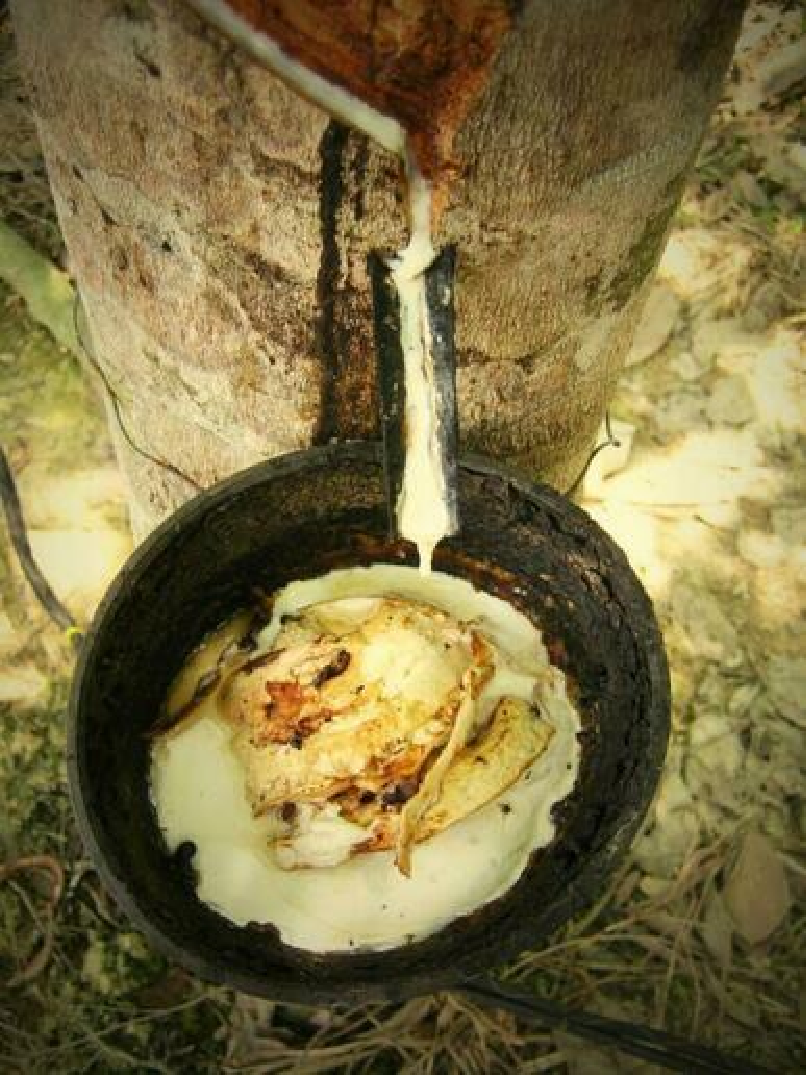
\includepdf[landscape=false,pages={1-1},nup=1x1,frame=false]{images/Test2-latex-001.pdf}
\end{lstlisting}

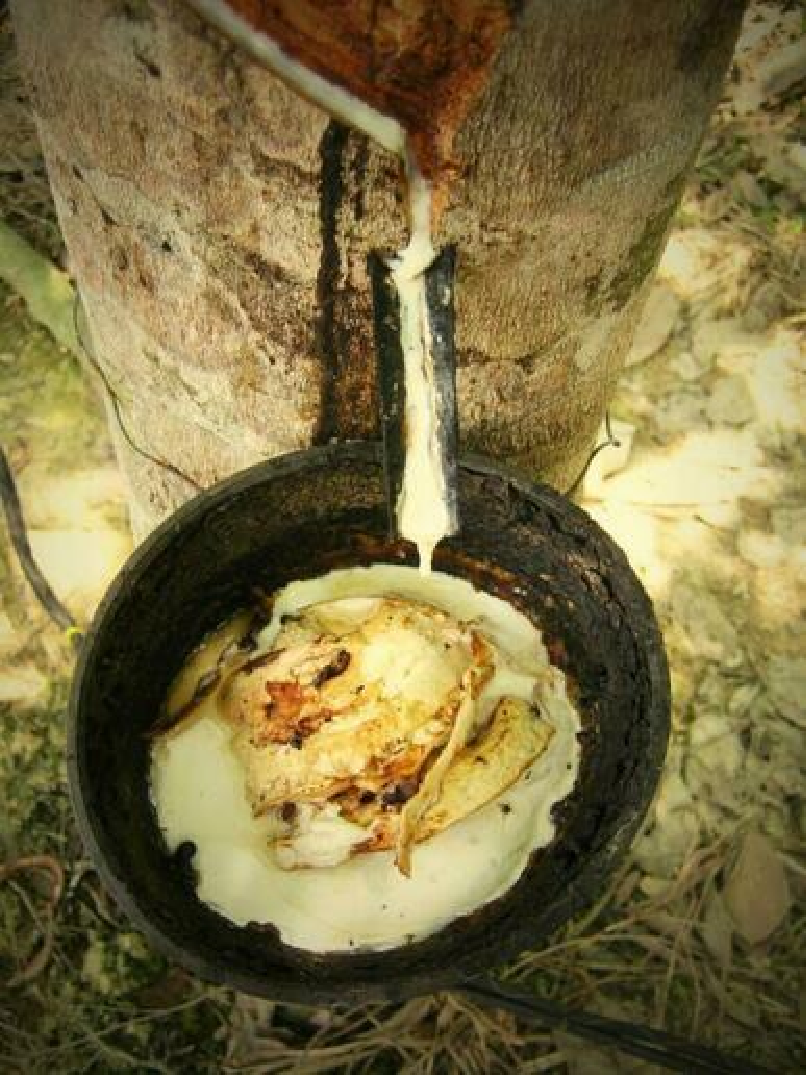
\includepdf[landscape=false,pages={1-1},nup=1x1,frame=false]{images/Test2-latex-001.pdf}

\clearpage
\subsection*{Stand der Forschung}

Während die traditionelle Latexproduktion bereits hinreichend erforscht ist (\ref{fig:latex}), bleibt das wissenschaftliche Verständnis elektronischer Verarbeitungsprozesse dieses vielseitigen Materials weiterhin lückenhaft. 


\begin{figure}[hb]
	\centering
	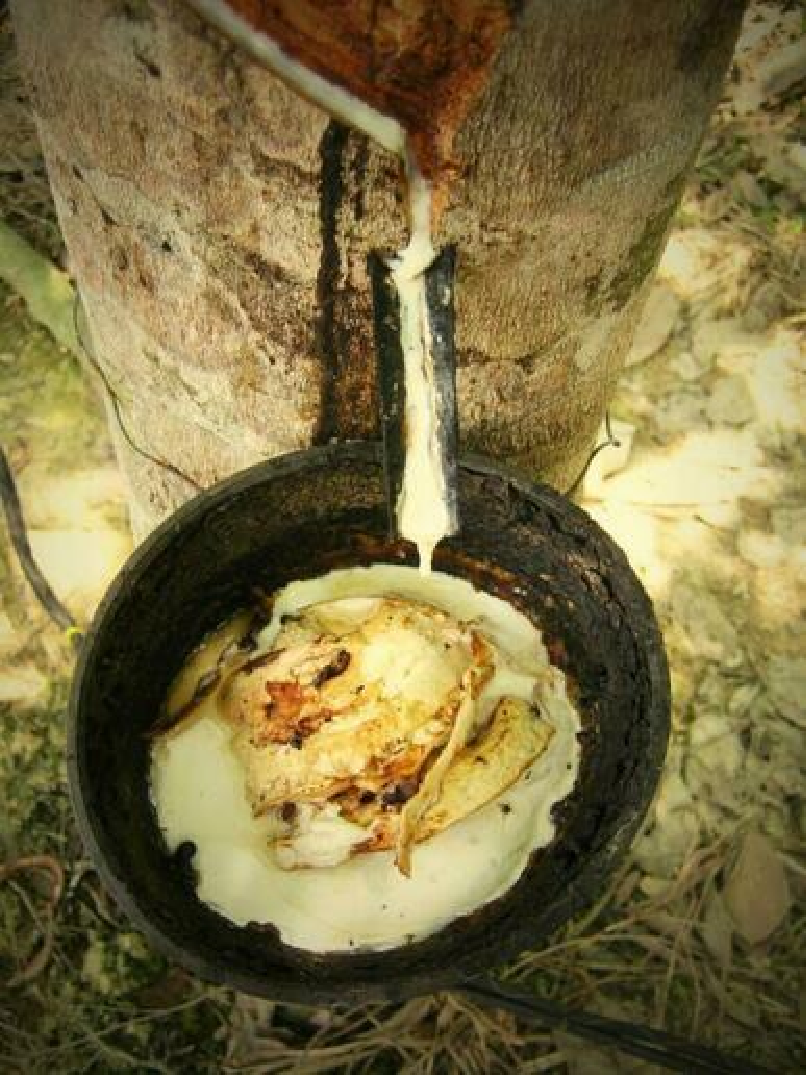
\includegraphics[width=0.35\textwidth]{images/Test2-latex-001.pdf}
	% -----------------------
	\caption{Traditionelle Latexproduktion}\label{fig:latex}%
\end{figure}
\marginpar{Abb.}


\begin{lstlisting}[language=TeX,% C, TeX, Bash, Python
]-----Code einfügen---------------------------%
	% Optionen
	scale = Wert, Vergrösserungsfaktor
	width/height = Wert für die Einstellung der Breite/Höhe
	angle = Wert, Winkel (in Grad)
	b = bottom - Seitenende 
	t = top - Seitenanfang
	h = here
	p = page - komplette Seite  
	
	\begin{figure}[hb]
	\centering
	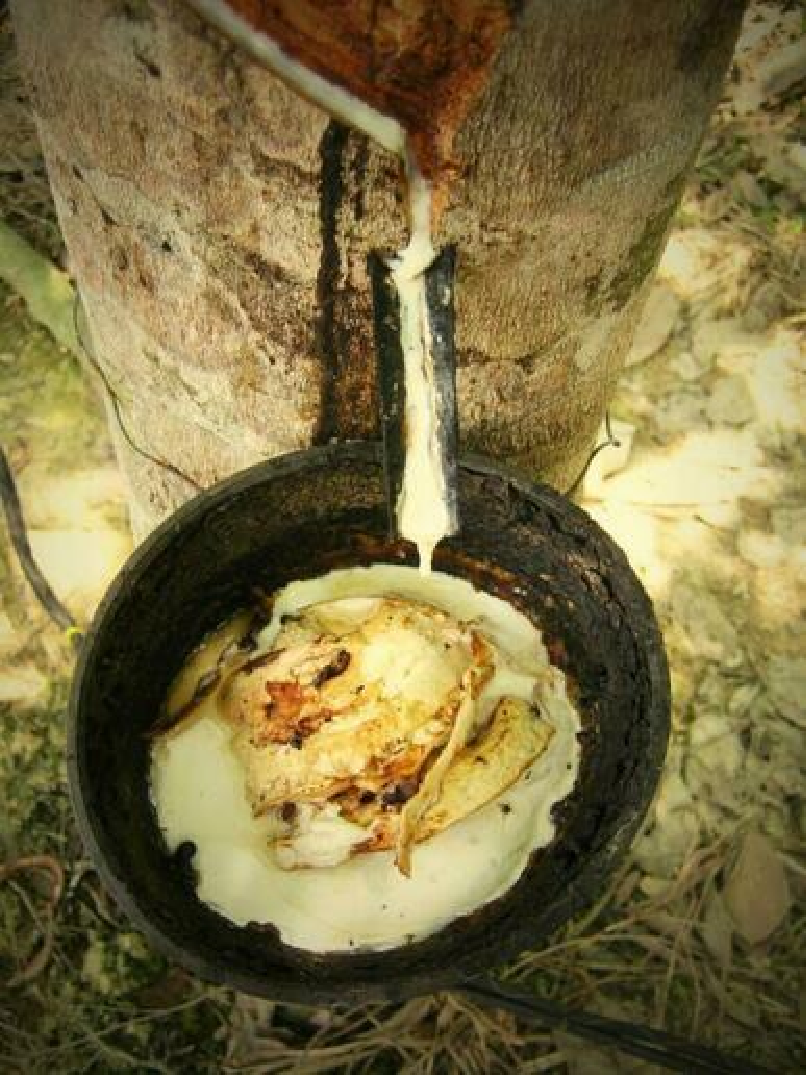
\includegraphics[width=0.35\textwidth]{images/Test2-latex-001.pdf}
	% -----------------------
	\caption{Traditionelle Latexproduktion}\label{fig:latex}%
	\end{figure}
\end{lstlisting}


\clearpage
\section*{Methodik}

Unter Zuhilfenahme der Formeln~\ref{eq:ekin} und \ref{eq:impuls} werden wir diese Forschungslücke schließen.  \marginpar{Mathe}
$E_\mathrm{kin}$ ist die kinetische Energie, $m$ die Masse und $\vec{v}$ die Geschwindigkeit.

Wurzel
$\sqrt{2}$

Bruch
$\frac{Zähler}{Nenner}$

\begin{equation}
% -----------------------
\label{eq:ekin}% 
\sum E_\mathrm{kin} = \sum E'_\mathrm{kin}
\end{equation}

\begin{equation}
% -----------------------
\label{eq:impuls}% 
\vec{v_1} - \vec{v_1'} = \frac{m_2}{m_1} (\vec{v_2'} - \vec{v_2})
\end{equation}

\clearpage
\section*{Ausblick}

Daraus ergeben sich gemäß (\ref{tab:schritte}) folgende nächste Schritte, deren sequenzielle Ausführung von essenzieller Bedeutung ist.

\begin{table}[ht]
	\centering
	\begin{tabular}{ll}% lcr
		\toprule
		\textbf{Nr.} & \textbf{Vorgehen} \\
		\midrule
		1 & Aktuellen Forschungsstand recherchieren \\
		2 & Methoden entwickeln \\
		3 & Schlussfolgerung aufstellen \\
		\bottomrule
	\end{tabular}
	% -----------------------
	\caption{Nächste Schritte}\label{tab:schritte}
\end{table}
\marginpar{Tabelle} 

\begin{lstlisting}[language=TeX,% C, TeX, Bash, Python
]-----Code einfügen---------------------------%
	\begin{table}[ht]
	\centering
	\begin{tabular}{ll}% lcr
	\toprule
	\textbf{Nr.} & \textbf{Vorgehen} \\
	\midrule
	1 & Aktuellen Forschungsstand recherchieren \\
	2 & Methoden entwickeln \\
	3 & Schlussfolgerung aufstellen \\
	\bottomrule
	\end{tabular}
	% -----------------------
	\caption{Nächste Schritte}\label{tab:schritte}
	\end{table}
\end{lstlisting}

%---------------------

%\clearpage
%\phantomsection\addcontentsline{toc}{chapter}{Literatur}
%\printbibliography% Verzeichnis drucken
\end{document}